\chapter{Implementation}

\section{Android x86}

\subsection{Scenario 1 - propagate underneath Dalvik VM}

Android x86 suffers from the same kind of vulnerabilities just like any other
system that runs on the x86 architecture does, stack overflow, heap overflow,
format string vulnerability, etc. Any app that leverages the power of native
library becomes a potential threat. To prove that \emph{CRAXDroid} is able to
generate exploit automatically on Android x86, a vulnerable app is constructed
intentionally.

\begin{figure}[!ht]
  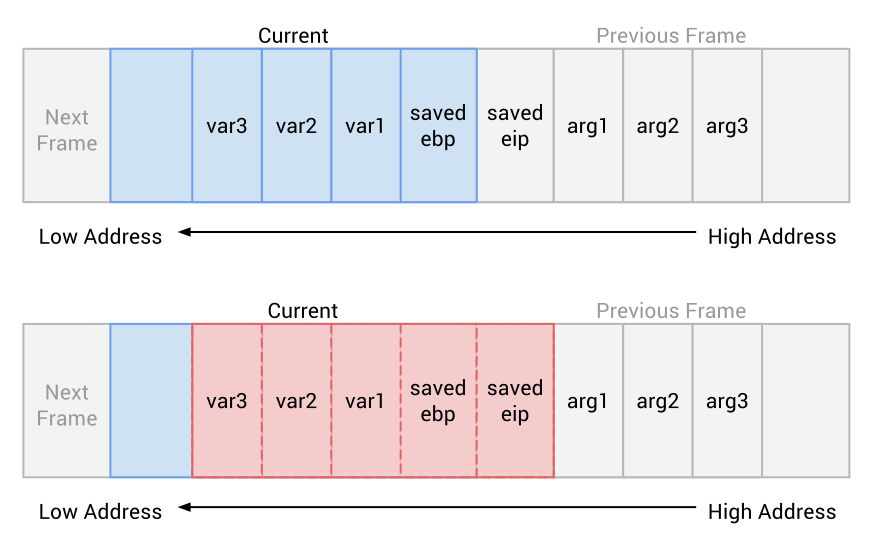
\includegraphics[width=\textwidth]{x86-stack-layout}
  \caption{x86 stack layout}
  \label{fig:x86-stack-layout}
\end{figure}

The vulnerable app contains a stack overflow vulnerability caused by improper
use of the function \textbf{strcpy}. \textbf{strcpy} is known to cause
stack overflow if boundary checking is not done properly. For example, copying
content of a buffer with 10 bytes to a buffer with only 5 bytes would overwrite
the stack by 5 bytes. Combining with the nature of x86 architecture, which
store instruction pointers (EIP) on the stack as shown in
Figure~\ref{fig:x86-stack-layout}, attackers would be able to forge the EIP
value and intrude the running process.

\emph{CRAXDroid} first maps a local file into memory by using \textbf{mmap} and
marks the part of the memory as symbolic to keep track of the flow of the file
content. After the vulnerable app is launched, the target file is opened and
read by the loaded native library. Since the file is mapped to a chunk of
memory, the content would be read from the chunk of memory instead of physical
hard drive. Once the process retrieves the saved instruction pointer from the
returning stack frame, a pre-deployed sensor set by \emph{CRAXDroid} would
check if the EIP is contaminated by the symbolic input and trigger the
progress of exploit generating if the examination goes true.

\subsection{Scenario 2 - propagate through Dalvik VM}

\section{ARM}
\subsection{Raspberry Pi}
\subsection{Linux ARM}
\subsection{Android ARM}

% vim: sw=2 sts=2 et
